% Figure T2, generated by experiments/t2_superposition.py.
\begin{figure}[t]
  \centering
  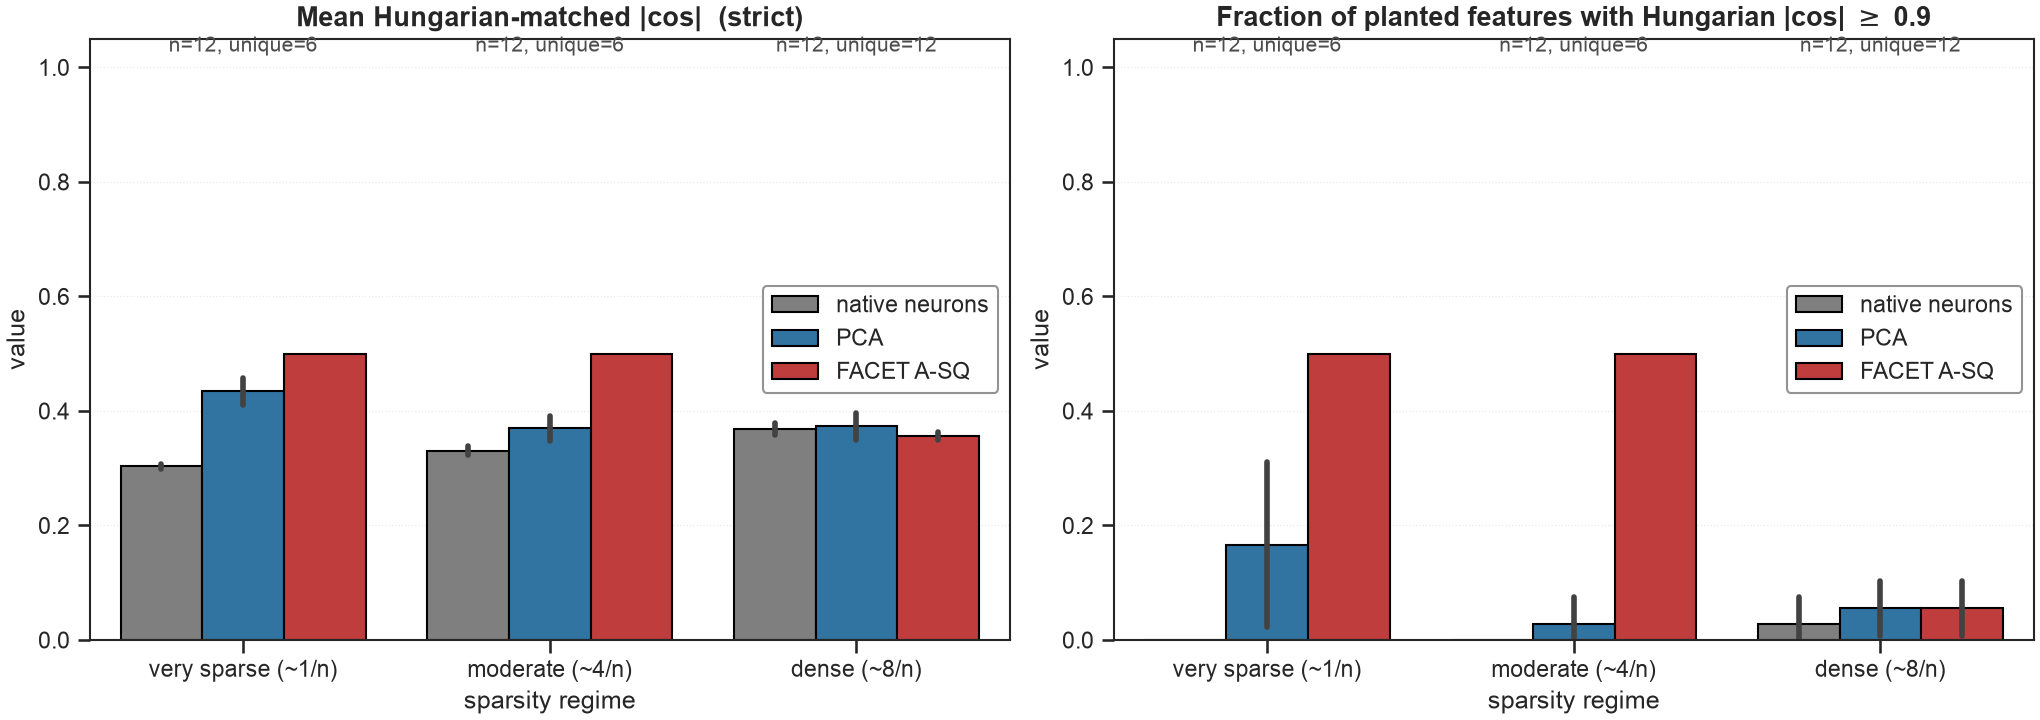
\includegraphics[width=\linewidth]{../shared/figures/generated/t2_superposition.png}
  \caption{\textbf{T2, controlled-neural bridge: feature recovery across three sparsity regimes.} Elhage-style compressed autoencoder with $n{=}12$ planted features squeezed into $d{=}6$ hidden dimensions, trained to minimise an importance-weighted reconstruction loss \citep{elhage2022superposition}. Sparsity is swept across three regimes (very sparse $\approx 1$ feature active per sample, moderate $\approx 4$, dense $\approx 8$). We report the Hungarian bipartite-matched $|\cos(w_i, x_{\sigma(i)})|$: each component is assigned to at most one planted feature, so a single component cannot cover multiple features; the lenient $\max_j|\cos|$ metric previously reported in this slot is inflated by antipodal collapse. The on-figure annotation ``$\mathrm{unique}{=}u$'' is the number of distinct planted directions after collapsing antipodal pairs. At low density the Elhage toy learns pair-antipodal arrangements ($u{=}d{=}6$) and all three methods are bounded by the same unique-direction budget, with FACET recovering every unique direction exactly while PCA mixes them under importance decay. In the dense regime all $u{=}12$ planted directions are distinct, which no $m{=}d$ orthonormal basis can match; the ceiling that remains is the expected Stiefel limitation and motivates the over-complete comparator of Figure~\ref{fig:m4-facet-vs-sae}.}
  \label{fig:t2-superposition}
\end{figure}
